% numerical.tex

\cleardoublepage
\chapter{Optimised Ascent Trajectory}\label{chapter:Ascent}

This chapter presents a maximum payload-to-orbit trajectory optimisation for the rocket-scramjet-rocket launch system incorporating the SPARTAN. 
The launch system is launched from the Equatorial Launch Australia launch site in East Arnhem Land, and delivers a small satellite into sun synchronous orbit. LODESTAR is used to calculate the trajectory solutions for multiple launch scenarios, and these trajectory solutions are investigated to gain insight into the optimised trajectory.

Firstly, a trajectory is calculated for the case in which the SPARTAN flies a constant dynamic pressure. This trajectory is calculated to serve as a baseline for comparisons to be made, as previous studies have assumed that flying the SPARTAN at its maximum allowable dynamic pressure would produce the best overall system performance[CITEXX]. An optimal payload-to-orbit trajectory is then developed, and the trajectory shape compared and contrasted to the constant dynamic pressure trajectory. Lastly, a sensitivity study is performed, varying key performance parameters of the launch system and investigating the effects of each parameter on the performance of the launch system. 

The following trajectories are developed: 
\begin{enumerate}
	\item: $q = $ 50kPa fixed SPARTAN trajectory with minimum pull-up. \newline$\rightarrow$ This trajectory provides a baseline trajectory for comparison purposes.
	\item: Trajectory optimised for payload-to-orbit, $q_{max} = $ 50kPa. \newline$\rightarrow$ This trajectory Demonstrates improved performance through coupled trajectory optimisation.
	\item: Variation of maximum allowable dynamic pressure between $q_{max} = $ 40kPa \& $q_{max} = $ 50kPa. 
	\newline$\rightarrow$ Comparison of these simulations allows investigation into the effect of $q$ max on payload-to-orbit, and enables inferences about the effects of variation in the structural strength of the SPARTAN.
	\item: Variation of the coefficient of drag of the SPARTAN between $C_d = 90\%$ \& $C_d = 110\%$. 
	\newline$\rightarrow$ Comparison of optimal trajectories with drag variation allows investigation of the robustness of the solution with variation in vehicle design, and allows inferences about the effects of vehicle shape on the efficiency of the system. 
	\item: Variation of the specific impulse of the SPARTAN's C-REST engines between $I_{SP} = 90\%$ \& $I_{SP} = 110\%$. 
	\newline$\rightarrow$ Comparison of optimal trajectories with specific impulse variation allows investigation of the effects of the efficiency of the C-REST engines on the efficiency of the system. 
	\item: Variation of the mass of the SPARTAN between $m_2 = 90\%$ \& $m_2 = 110\%$. 
	\newline$\rightarrow$ Comparison of optimal trajectories with SPARTAN mass variation allows investigation of the effects of the SPARTAN design on the launch system efficiency, and allows inferences about the effect of the internal layout of the SPARTAN. 
	\item: Variation of the fuel mass of the SPARTAN between $m_{fuel} = 90\%$ \& $m_{fuel} = 110\%$. 
	\newline$\rightarrow$ Comparison of optimal trajectories with SPARTAN fuel mass variation allows investigation of the effects of the amount of fuel which the SPARTAN is able to carry on the launch system efficiency. 
	\item: Variation of the mass of the third stage rocket between $m_3 = 90\%$ \& $m_3 = 110\%$. 
	\newline$\rightarrow$ Comparison of optimal trajectories with third stage mass variation allows investigation of the effects of the third stage design on the efficiency of the launch system, and allows inferences about the effects of the third stage internal layout on the efficiency of the system. 
	\item: Variation of the thrust of the third stage rocket between $T_3 = 90\%$ \& $T_3 = 110\%$. 
	\newline$\rightarrow$ Comparison of optimal trajectories with third stage thrust variation allows investigation of the effects of the output of the third stage engine on the efficiency of the launch system. 
\end{enumerate}

\section{Constant Dynamic Pressure Trajectory}
\begin{figure}[ht]
	\centering
	\includegraphics[width=1\linewidth]{../LODESTAR_FINAL/Results/20180827T120326mode900/GroundTrackConstq}
	\caption{}
	\label{fig:GroundTrackConstq}
\end{figure}

The first trajectory which is produced using LODESTAR is a trajectory in which the SPARTAN flies a constant dynamic pressure path, at its maximum allowable dynamic pressure of 50kPa.
A constant dynamic pressure trajectory is produced to serve as a baseline for comparison with the maximum payload-to-orbit optimised trajectory, and to verify that LODESTAR is able to calculate a trajectory in which the SPARTAN flies at constant dynamic pressure. It is crucial to verify that the SPARTAN is able to be simulated to fly at constant dynamic pressure, as the aerodynamics and design of the vehicle have been changed from previous studies[CITEXX]. It must be ensured that any deviations from a constant dynamic pressure path in the payload-to-orbit optimised trajectory serve to improve the performance of the system, rather than being a result of the problem setup or design constraints. 

 In order to drive the SPARTAN towards a constant dynamic pressure path, the cost function described in Table \ref{tab:SPARTANascentsetup} is utilised. The maximum payload-to-orbit cost function is also active on the third stage phase, so that when the SPARTAN is close to 50kPa, the third stage will fly a maximum payload-to-orbit trajectory from the termination of the SPARTAN's constant dynamic pressure path. 

LODESTAR is able to successfully simulate the trajectory of the rocket-scramjet-rocket system, with the SPARTAN flying at constant dynamic pressure, achieving a payload-to-orbit of \PayloadToOrbitConstq kg.
Figure \ref{fig:GroundTrackConstq} shows the simulated trajectory path, and Table \ref{tab:constqsummary} provides a summary of the key trajectory parameters of the trajectory. 



\begin{table}[ht]
	\centering
	

\begin{tabular}{l c} 
	\hline \textbf{Trajectory Condition}
	&
	\\
	\hline \textbf{Payload to Orbit (kg)}
	& \PayloadToOrbitConstq
	\\
	\textbf{Separation Alt, 1$\rightarrow$2 (km)}
	& \firstsecondSeparationAltConstq
	\\
	\textbf{1$^{st}$ Stage Structural Mass Fraction}
	& \FirstStageSMFConstq
	\\
	\textbf{Separation Alt, 2$\rightarrow$3 (km)}
	& \secondthirdSeparationAltConstq
	\\
	\textbf{Separation $v$, 2$\rightarrow$3 (m/s)}
	& \secondthirdSeparationvConstq
	\\
	\textbf{Separation $\gamma$, 2$\rightarrow$3 (deg)}
	& \secondthirdSeparationgammaConstq
	\\
	\textbf{Separation $q$, 2$\rightarrow$3(kPa)}
	& \secondthirdSeparationqConstq
	\\
	\textbf{2$^{nd}$ Stage L/D, 2$\rightarrow$3}
	& \secondthirdSeparationLDConstq
	\\
	\textbf{2$^{nd}$ Stage Flight Time (s)}
	& \secondFlightTimeConstq
	\\
	\textbf{3$^{rd}$ Stage $t$, $q >$ 5kpa (s)}
	& \thirdqOverFiveConstq
	\\
	\textbf{3$^{rd}$ Stage $t$, max $\alpha$ (deg)}
	& \thirdmaxAoAConstq
	\\
	\textbf{3$^{rd}$ Stage final v (m/s)}
	& \thirdcircvConstq
	\\
	\hline 
\end{tabular} 
\caption{}
\label{tab:constqsummary}
\end{table}





\subsection{First Stage}
\begin{figure}[ht]
\centering
\includegraphics[width=1\linewidth]{../LODESTAR_FINAL/Results/20180827T120326mode900/FirstStageConstq}
\caption{}
\label{fig:FirstStageConstq}
\end{figure}

The rocket-scramjet-rocket system launches vertically, flying a fixed vertical trajectory for Xs, after which a pitchover is initiated. Under power of the first stage rocket, the launch system begins pitching, flying north-west, over the Arafura Sea. 
After pitchover the angle of attack stays constant at 0$^\circ$ for XXs. The angle of attack is reduced at XX s, reaching a minimum of XX, before increasing back up to 0$^\circ$ for stage separation. 
The SPARTAN is separated at an angle of XX, at an altitude of XXkm, a total flight time of XXs, with a total ground distance of XXkm covered under power of the first stage rocket. 



\subsection{Second Stage}

\begin{figure}[ht]
\centering
\includegraphics[width=1\linewidth]{../LODESTAR_FINAL/Results/20180827T120326mode900/SecondStageConstq}
\caption{}
\label{fig:SecondStageConstq}
\end{figure}


The constant dynamic pressure trajectory for the SPARTAN stage is shown in Figure \ref{fig:SecondStageConstq} with key results summarised in Table \ref{tab:constqsummary}. After the separation of the first stage rocket, the SPARTAN flies north west over the Arafura Sea, and crosses West Papua before releasing the third stage rocket. Due to the clear objective of a constant dynamic pressure trajectory, any deviations from the target dynamic pressure are readily apparent, allowing the efficacy of the optimiser to be verified. 
These results show very close adherence to 50kPa dynamic pressure (maximum XX\% deviation). Third stage release occurs at XX s at XX km altitude. 
Over the trajectory the Mach no. increases from XX to XX and the velocity from XXm/s to XX m/s. The flap deflection shows an overall increase from $XX^\circ$ to $XX^\circ$ over the trajectory.  The net specific impulse ($I_{sp_{net}} = \frac{T-D}{\dot{m}_f g}$) generally decreases over the trajectory, as the efficiency of the scramjet engines decreases. However, at the beginning of the trajectory the equivalence ratio increases as the capture limitations are relaxed with increasing Mach number. This causes the net specific impulse to increase, to a maximum of XX, during the first XXs flight time. 

\begin{figure}[ht]
	\centering
	\includegraphics[width=0.8\linewidth]{../LODESTAR_FINAL/Results/20180827T120326mode900/NetIspConstq}
	\caption{}
	\label{fig:NetIspConstq}
\end{figure}

\subsection{Third Stage}

\begin{figure}[ht]
\centering
\includegraphics[width=1\linewidth]{../LODESTAR_FINAL/Results/20180827T120326mode900/ThirdStageConstq}
\caption{}
\label{fig:ThirdStageConstq}
\end{figure}

Figure \ref{fig:ThirdStageConstq} shows the corresponding third stage atmospheric exit trajectory after release, evaluated as described in Chapter \ref{chapter:LODESTAR}. The third stage released from a constant dynamic pressure trajectory, shown in Figure XX, is limited by the maximum thrust vector angle for the first XXs of flight. This places significant limitations on the maximum allowable angle of attack. This angle of attack limitation reduces the lift of the rocket, causing it to spend a large amount of time at low altitude, in a high drag environment. The angle of attack increases gradually to a maximum of XX$^\circ$ at XXs before decreasing until burnout at XXs. The third stage rocket reaches XX dynamic pressure at XXs, and the heat shield is discarded. The rocket coasts to a trajectory angle of 0$^\circ$, which is reached at a total flight time of XXs. The trajectory terminates at 90km, the lowest allowable altitude for circularisation. 
When this altitude is reached, the trajectory is circularised and performs a Hohmann transfer manoeuvre to reach sun synchronous orbit.








\section{Optimised Ascent Trajectory}

This section presents the maximum payload-to-orbit trajectory for the rocket-scramjet-rocket launch system. 
The maximum payload-to-orbit trajectory shape is shown in Figure \ref{fig:GroundTrackStandardNoReturn}, and involves flying the SPARTAN away from its maximum dynamic pressure at multiple points along the trajectory, with altitude raising manoeuvres. These manoeuvres serve either to increase the net specific impulse of the SPARTAN, or to trade-off the efficiency of the SPARTAN in order to increase the efficiency of the first and third stages. 

\begin{figure}[ht]
	
	
	
	\centering
	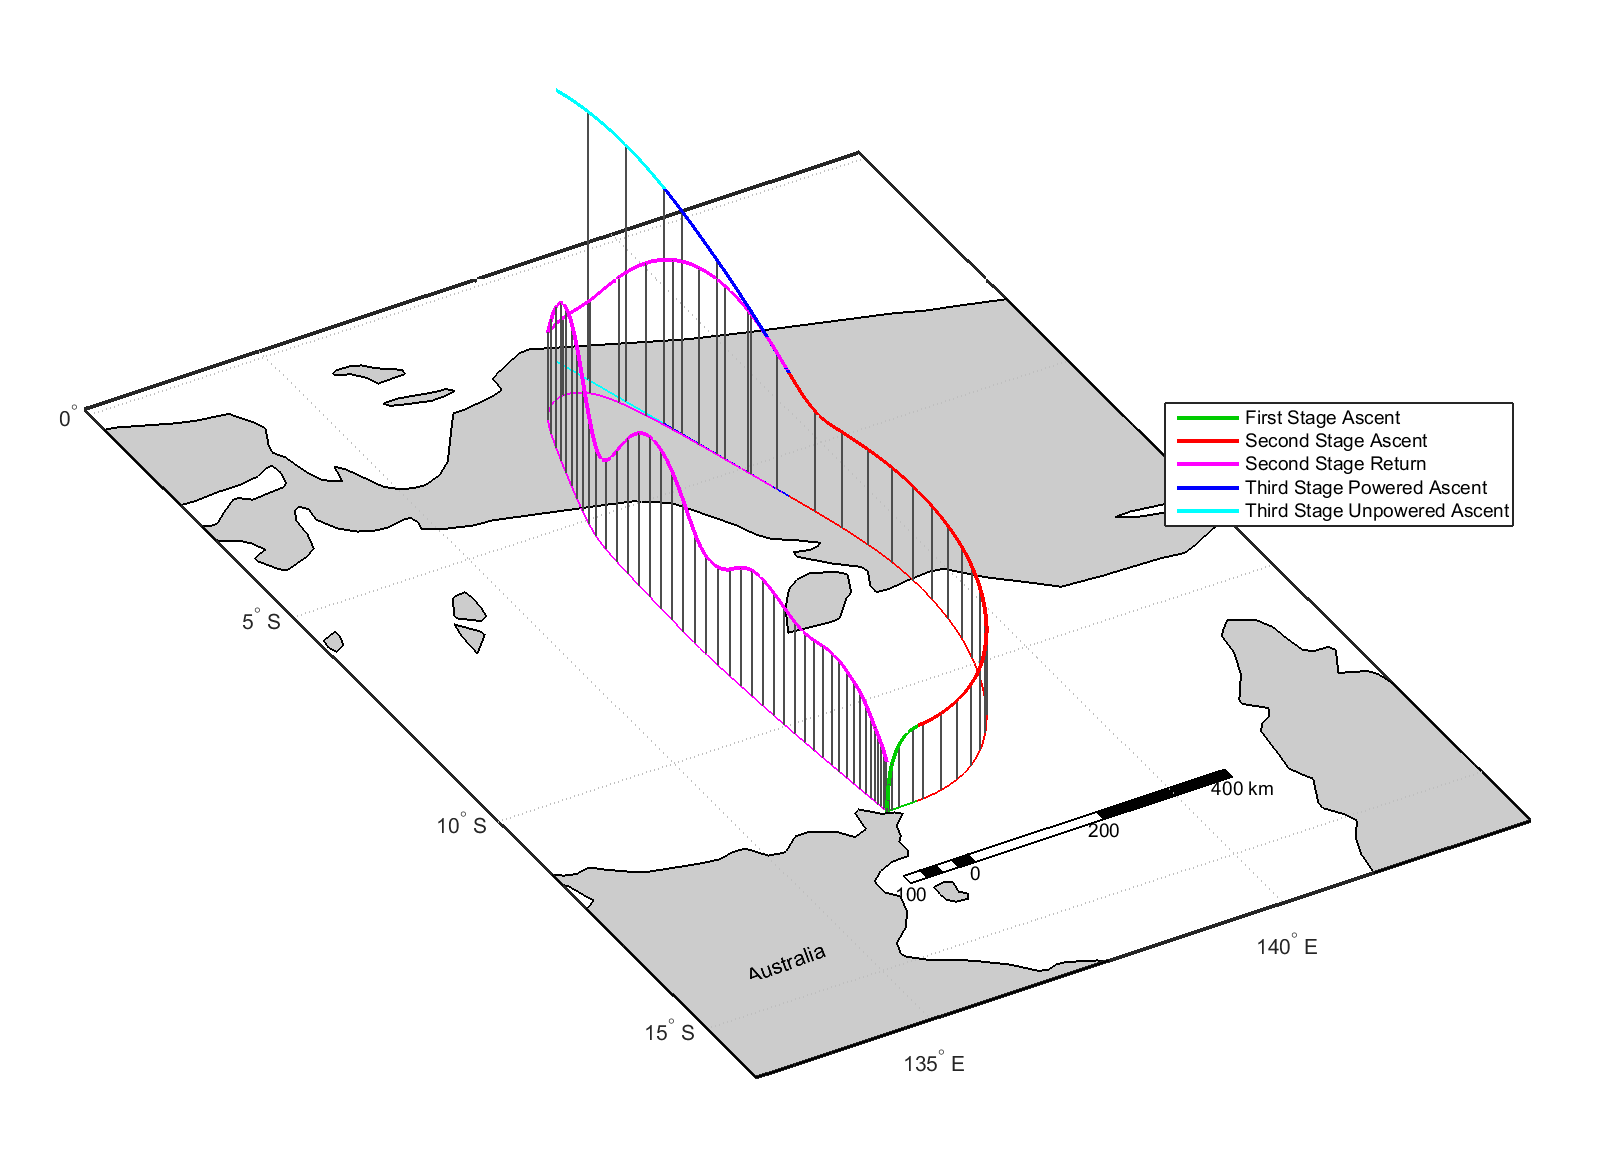
\includegraphics[width=1\linewidth]{../LODESTAR_FINAL/Results/mode10/GroundTrackStandard}
	\caption{}
	\label{fig:GroundTrackStandardNoReturn}
\end{figure}

Initially, the SPARTAN is released at a dynamic pressure of 50kpa. However, the trajectory angle at release is 3.13$^\circ$, which causes the altitude of the SPARTAN to immediately increase, and consequently for its dynamic pressure to decrease. This trajectory angle at release is the consequence of a trade-off of the efficiency of the SPARTAN for first stage efficiency. In order to release the SPARTAN at a lower trajectory angle, the first stage must launch with a lower fuel mass, to allow it to pitch in the correct manner. During the maximum payload-to-orbit trajectory, the first stage launches with a fuel mass of 17185kg, in contrast to the first stage segment of the constant dynamic pressure trajectory, which launches with a fuel mass of 17010kg in order to release the SPARTAN at a trajectory angle low enough to sustain constant dynamic pressure flight. Neither first stage utilises the full amount of allowable fuel mass, 17934kg, indicating that using the full fuel mass would reduce the efficiency of the SPARTAN unfavourably. 
During the maximum payload-to-orbit trajectory, the first stage rocket releases the SPARTAN at a velocity of 1484.3m/s, in contrast to the first stage releasing the SPARTAN onto a constant dynamic pressure trajectory, which separates the SPARTAN at a velocity of 1466.5m/s. 
These complex interactions indicate that the fuel mass that the first stage utilises has a distinct optimal magnitude, and that the design of the first stage may have substantial influence on the optimal trajectory shape. 

\begin{table}[ht]
	\centering
	\begin{tabular}{l c c c c c} 
		\hline \textbf{Trajectory Condition}
		&Standard
		\\
		\hline \textbf{Payload to Orbit (kg)}
		& \PayloadToOrbitStandardNoReturn
		\\
		\textbf{Separation Alt, 1$\rightarrow$2 (km)}
		& \firstsecondSeparationAltStandardNoReturn
		\\
		\textbf{1$^{st}$ Stage Structural Mass Fraction}
		& \FirstStageSMFStandardNoReturn
		\\
		\textbf{Separation Alt, 2$\rightarrow$3 (km)}
		& \secondthirdSeparationAltStandardNoReturn
		\\
		\textbf{Separation $v$, 2$\rightarrow$3 (m/s)}
		& \secondthirdSeparationvStandardNoReturn
		\\
		\textbf{Separation $\gamma$, 2$\rightarrow$3 (deg)}
		& \secondthirdSeparationgammaStandardNoReturn
		\\
		\textbf{Separation $q$, 2$\rightarrow$3(kPa)}
		& \secondthirdSeparationqStandardNoReturn
		\\
		\textbf{2$^{nd}$ Stage L/D, 2$\rightarrow$3}
		& \secondthirdSeparationLDStandardNoReturn
		\\
		\textbf{2$^{nd}$ Stage Flight Time (s)}
		& \secondFlightTimeStandardNoReturn
		\\
		\textbf{3$^{rd}$ Stage $t$, $q >$ 5kpa (s)}
		& \thirdqOverFiveStandardNoReturn
		\\
		\textbf{3$^{rd}$ Stage $t$, max $\alpha$ (deg)}
		& \thirdmaxAoAStandardNoReturn
		\\
		\hline \textbf{3$^{rd}$ Stage final v (m/s)}
		& \thirdcircvStandardNoReturn
		\\
		\hline 
	\end{tabular} 
	\label{tab:summaryStandardNoReturn}
\end{table}



\subsection{First Stage}
\begin{figure}[ht]
\centering
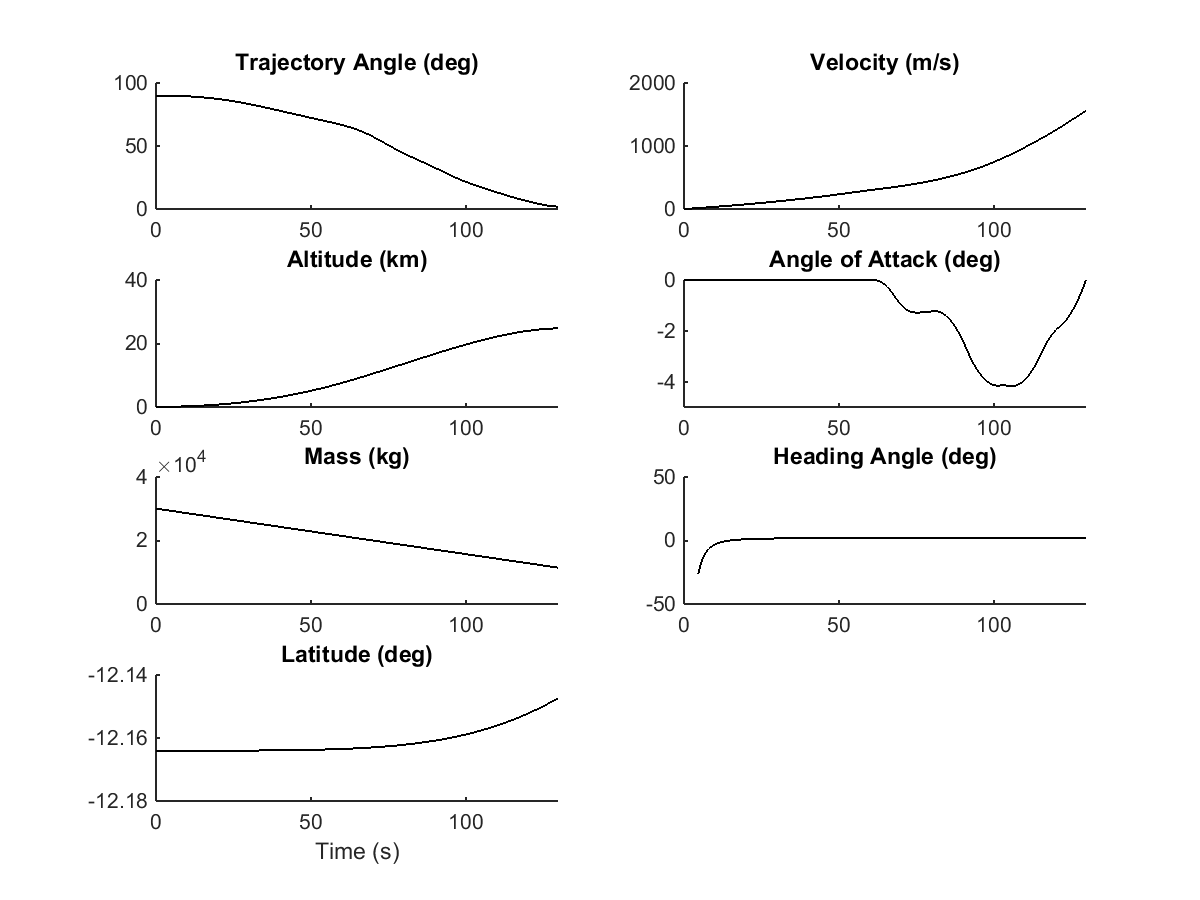
\includegraphics[width=1\linewidth]{../LODESTAR_FINAL/Results/mode10/FirstStageStandard}
\caption{}
\label{fig:FirstStageStandardNoReturn}
\end{figure}

\subsection{Second Stage}
\begin{figure}[ht]
\centering
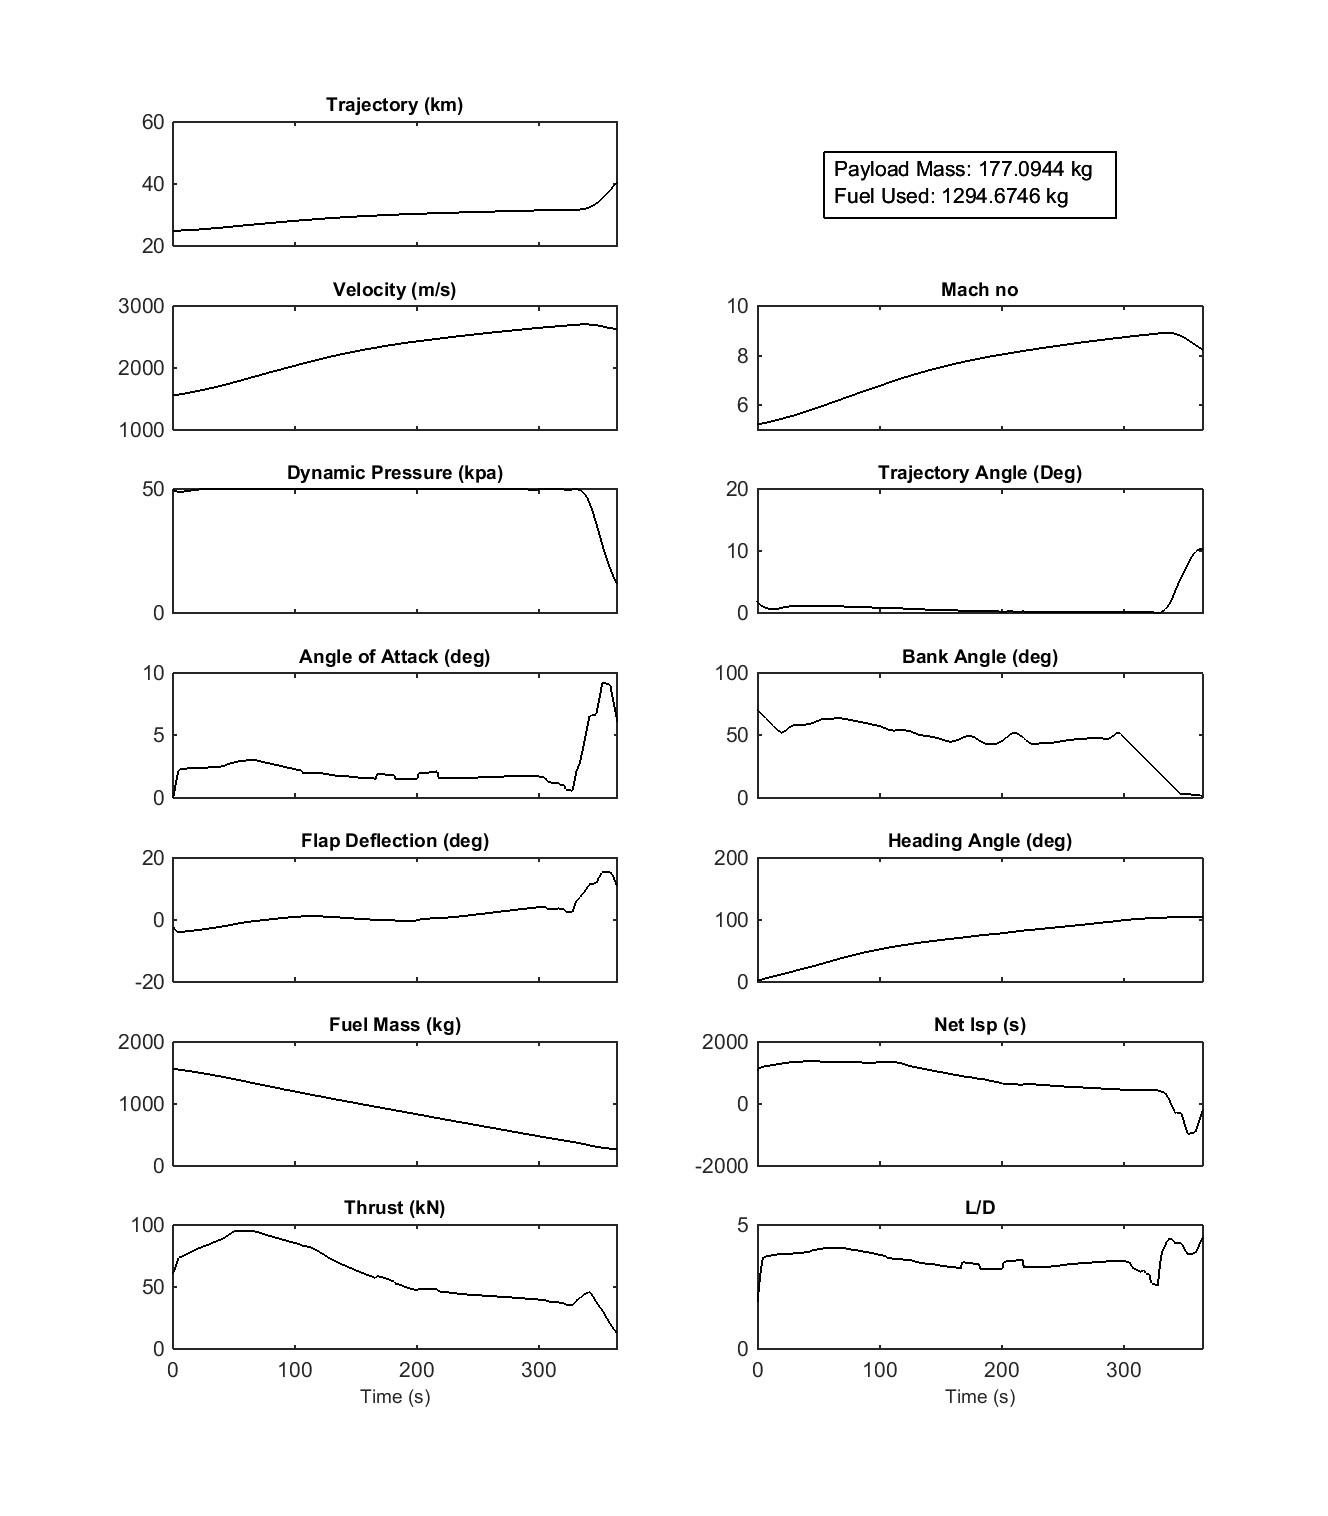
\includegraphics[width=1\linewidth]{../LODESTAR_FINAL/Results/mode10/SecondStageStandard}
\caption{\textcolor{red}{maybe plot equivalence ratio to compare}}
\label{fig:SecondStageStandardNoReturn}
\end{figure}




At 122.5 seconds, the altitude of the trajectory is raised, and the dynamic pressure decreased, to a minimum of 35.6kPa. In this region the net specific impulse of the SPARTAN is fairly homogeneous, which can be observed in Figure \ref{fig:NetIspStandardNoReturn}. This is caused by the homogeneity which can be observed in the specific impulse of the C-REST engines in Figure \ref{fig:IspStandard}, between M1 values of 6 and 7. This homogeneity means that flying at the maximum dynamic pressure in this region does not necessarily produce the maximum specific impulse from the C-REST engines. As a result, this manoeuvre results in a slight increase the in the net specific impulse of the SPARTAN





LODESTAR is configured to optimise the total payload mass to orbit.
A maximum dynamic pressure limit of 50kPa is applied to the optimisation process to allow direct comparison with the constant $q$ trajectory and so that an equivalent vehicle can be used.   


The optimal trajectory shape for a $q=$50kPa limited, maximum payload to orbit trajectory is shown in Figure \ref{fig:SecondStageStandardNoReturn} with key results summarised in Table \ref{tab:summaryStandardNoReturn}. 
The equivalence ratio of the engine is less than 1 until XX,

 causing the SPARTAN to fly under 50kPa in this region (to a minimum of XXkPa) in order to raise equivalence ratio by flying in a higher temperature region. 

This increase in equivalence ratio results in a corresponding increase in net specific impulse.
After the equivalence ratio increases to 1, the trajectory follows a constant dynamic pressure path at 50kPa until XXs at which point a pull-up manoeuvre is performed, gaining altitude until rocket stage release at XXs flight time. 
This trajectory is able to deliver XXkg of payload to heliocentric orbit, an increase of XX over the constant dynamic pressure result with minimum pull-up. The point at which the pull-up manoeuvre begins is the optimisation result that takes into account the best combination of velocity, altitude and release angle for scramjet stage performance and the release of the rocket stage. This pull-up indicates the region at which increasing altitude and release angle becomes more important than extracting maximum thrust from the scramjet (which is generally attained at high $q$ and low flight angle at an equivalence ratio of 1).
Flight in a lower dynamic pressure environment results in less thrust output from the scramjet engines, as well as an increase in angle of attack and flap deflection angle to compensate for the additional lift required. Due to this, less overall acceleration is obtained compared to the constant dynamic pressure result with minimum pull-up. Separation occurs at a velocity of XXm/s, a decrease of XXm/s. However, at the same time separation altitude increases by XXkm to XXkm, resulting in a decrease in separation dynamic pressure to XXkPa. 

The larger scramjet stage pull-up assists the rocket in manoeuvring to exoatmospheric altitude by increasing the altitude and angle at separation by virtue of the increased L/D ratio and manoeuvrability of the scramjet vehicle. Even a small increase in release angle, to the optimal angle of XX$^\circ$, significantly reduces the turning that is required by the rocket as evident from comparing Fig \ref{fig:ThirdStageConstq} and \ref{fig:ThirdStageStandardNoReturn}. Further benefits are the reduced time that the rocket must spend in a high dynamic pressure environment, and a decrease in the maximum dynamic pressure that the rocket stage experiences by XX. This allows the structural mass and heat shielding, necessary to achieve exoatmospheric flight, to be decreased, enabling higher payload to orbit. 


Compared to studies considering vehicles with a scramjet-rocket transition within a single stage\cite{Lu1993}\cite{Trefny1999}, the maximum payload to orbit trajectory of the multi-stage system shows a scramjet-rocket transition point at much lower altitudes.
This lower transition point is a consequence of the stage separation creating an energy trade-off, which does not occur in a single stage vehicle. Single-stage vehicles must necessarily transport all components to exoatmosphere, and so utilise the scramjet engines until higher altitude to take advantage of their high efficiency. A multi-stage vehicle is able to separate the scramjet stage. 
This separation occurs when the performance benefits provided by the superior aerodynamics and engine efficiency of the scramjet stage are offset by the energy required to lift the extra mass to higher altitude. The beneficial ability
to separate the scramjet stage results in a lower altitude scramjet-rocket transition point, when compared to single
stage vehicle designs.




\begin{figure}[ht]
	\centering
	\includegraphics[width=0.8\linewidth]{../LODESTAR_FINAL/Results/mode10/NetIspStandard}
	\caption{}
	\label{fig:NetIspStandardNoReturn}
\end{figure}

\begin{figure}
\centering
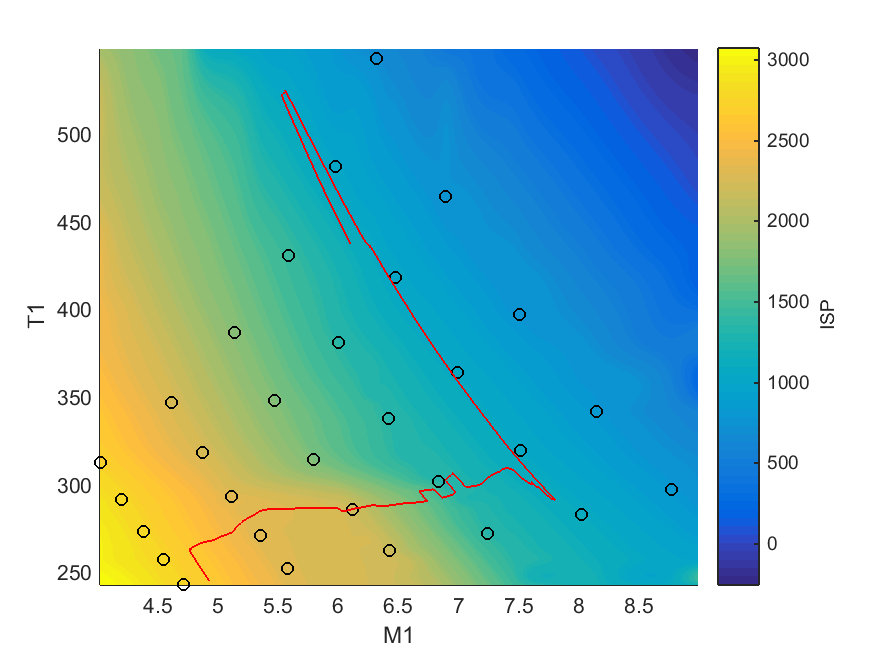
\includegraphics[width=0.7\linewidth]{../LODESTAR_FINAL/Results/mode10/IspStandard}
\caption{}
\label{fig:IspStandard}
\end{figure}

\subsection{Third Stage}

\begin{figure}[ht]
\centering
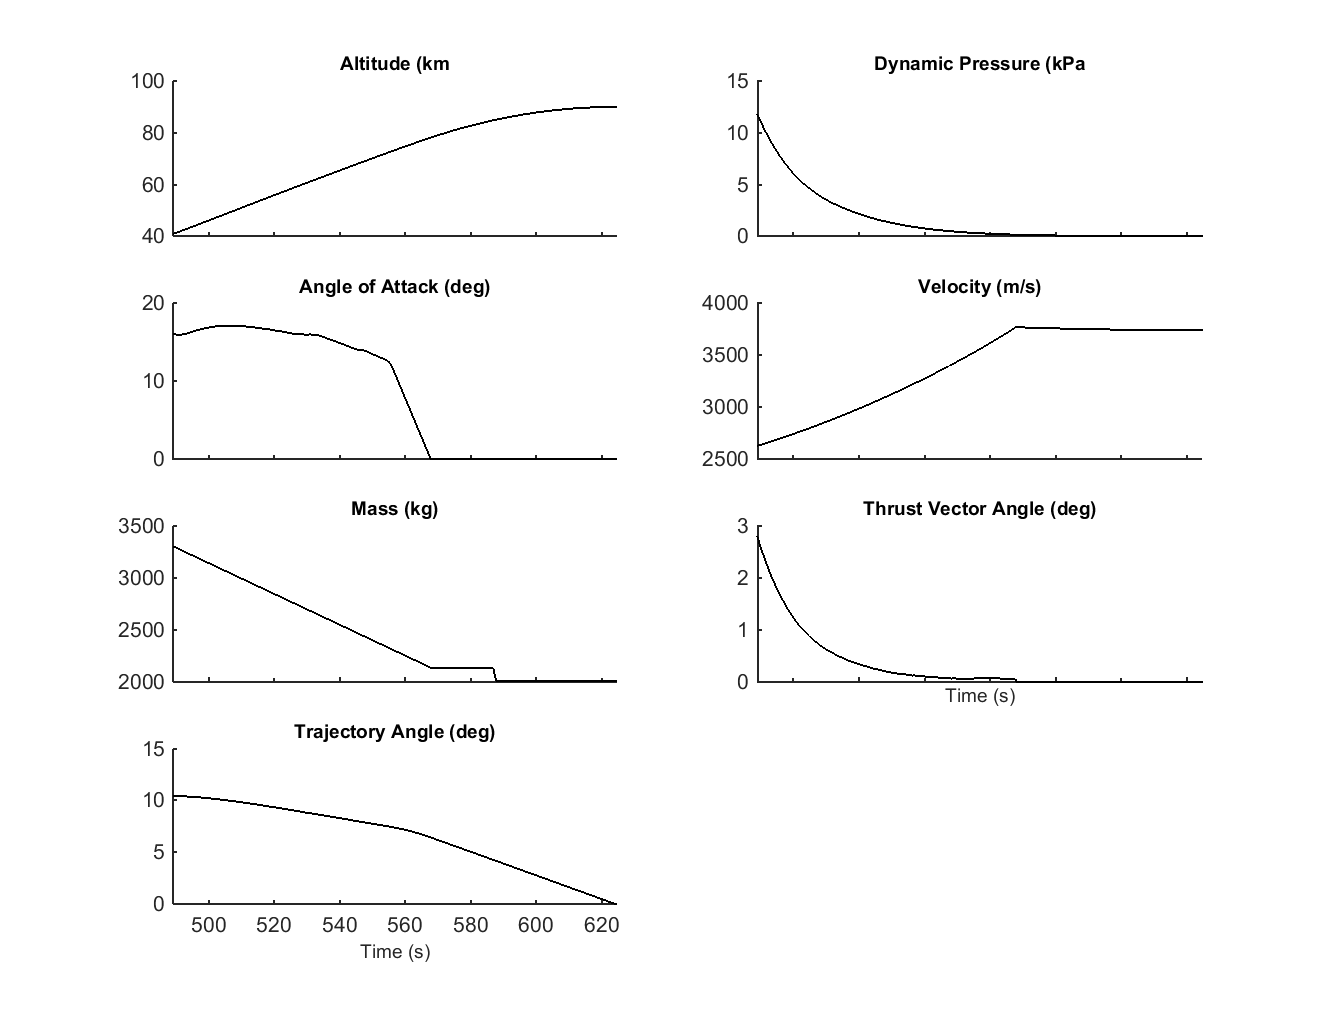
\includegraphics[width=1\linewidth]{../LODESTAR_FINAL/Results/mode10/ThirdStageStandard}
\caption{}
\label{fig:ThirdStageStandardNoReturn}
\end{figure}

-third stage spends much less time at high q, has much lower max q. mention heating relationship to q?


The release of the third stage rocket from an optimised scramjet trajectory is shown in Figure XX. Release at a higher, more optimal angle, mitigates the effects of the thrust vector angle limitation, so that the thrust vector limit is only reached during the first XXs flight time. After this, the angle of attack is limited by the maximum allowable normal force rather than the thrust vector limit, resulting in a higher maximum angle of attack. The rocket increases flight path angle and gains altitude rapidly, resulting in less time spent in a high drag environment, and a larger payload to orbit.  The angle of attack is increased gradually to XX$^\circ$ at XXs, before decreasing until burnout at XXs.


\section{Sensitivity Analysis}


\subsection{Dynamic Pressure Sensitivity}\label{sec:qvariation}

To investigate the sensitivity of the vehicle to changes in $q_{max}$, the maximum dynamic pressure is varied to XXkPa and the flight trajectory optimised, with results shown in XX.
The $XX\%$ variation in maximum dynamic pressure has XX effect on the payload mass delivered to heliocentric orbit.  Varying the maximum dynamic pressure by $\pm$XXkPa from 50kPa causes a variation of only  XX (XX) or XX (XX) in payload to orbit.  
Separation altitudes of XX km and XX km are reached for XXkPa and XXkPa limited cases respectively, with separation velocities of XX m/s and XX m/s. The XXkPa limited case flies for XXs, significantly longer than the XXkPa case which flies for XXs.
Both trajectories pull-up to similar altitudes, with relatively small variation in separation velocity XXm/s or XXm/s).
This small variation in velocity is despite the increase in air density and decrease in angle of attack required for flight at XXkPa dynamic pressure, both of which increase the mass flow into the engine. Although the thrust output of the REST engines increases with dynamic pressure, so does the drag on the vehicle, and the net increase in performance is small. 


Only a small variation in optimal payload mass is observed, without modification of vehicle design to account for the dynamic pressure limit. This indicates that designing and operating a vehicle at lower dynamic pressures may be preferable. Flying at a lower maximum dynamic pressure allows reduction of the structural weight and heat shielding of the vehicle. However, as the XXkPa limited case has a higher first-second stage separation altitude, a larger first stage fuel mass is required, though this increase in fuel mass is small. Between XXkm  and XXkm (XXkPa and XXkPa optimal start points) there is only a XX\% variation in the fuel mass required. This small variation in first stage fuel consumption would easily be offset by a decrease in second stage structural mass. 


\subsection{Drag Sensitivity Analysis}\label{sec:dragvariation}


To investigate the effect of vehicle design and uncertainty in aerodynamic performance on the optimal trajectory the drag on the vehicle is varied by XX\%, and an optimised trajectory calculated with dynamic pressure limited to 50kpa. Selected results are compared to the 100\% drag result in XX. 
These results show that when drag is increased (ie. L/D is decreased) the optimal trajectory shape is similar to the base-line case, though the high drag second stage follows a slightly slower and hence lower flight path, with a lower stage transition point. The similar flight path shape of the high drag case suggests that sacrificing velocity to increase separation altitude in a pull-up manoeuvre is optimal for multiple vehicle designs. Although the lower transition point indicates that the rocket is favoured at an earlier point in the climb manoeuvre, due to the decreased aerodynamic efficiency of the scramjet vehicle. 
The net result is  a lower payload-to-orbit of XXkg (a decrease of XX\%). 

\begin{tabular}{l c c c c c c} 
	\hline \textbf{Trajectory Condition}
	&Cd90
	&Cd95
	&Cd100
	&Cd105
	&Cd110
	& /\%
	\\
	\hline \textbf{Payload to Orbit (kg)}
	& \PayloadToOrbitCdNinetyNoReturn
	& \PayloadToOrbitCdNinetyFiveNoReturn
	& \PayloadToOrbitCdStandardNoReturn
	& \PayloadToOrbitCdOneHundredFiveNoReturn
	& \PayloadToOrbitCdOneHundredTenNoReturn
	&-1.9
	\\
	\textbf{Separation Alt, 1$\rightarrow$2 (km)}
	& \firstsecondSeparationAltCdNinetyNoReturn
	& \firstsecondSeparationAltCdNinetyFiveNoReturn
	& \firstsecondSeparationAltCdStandardNoReturn
	& \firstsecondSeparationAltCdOneHundredFiveNoReturn
	& \firstsecondSeparationAltCdOneHundredTenNoReturn
	&-0.09
	\\
	\textbf{Separation Alt, 2$\rightarrow$3 (km)}
	& \secondthirdSeparationAltCdNinetyNoReturn
	& \secondthirdSeparationAltCdNinetyFiveNoReturn
	& \secondthirdSeparationAltCdStandardNoReturn
	& \secondthirdSeparationAltCdOneHundredFiveNoReturn
	& \secondthirdSeparationAltCdOneHundredTenNoReturn
	& -
	\\
	\textbf{Separation $v$, 2$\rightarrow$3 (m/s)}
	& \secondthirdSeparationvCdNinetyNoReturn
	& \secondthirdSeparationvCdNinetyFiveNoReturn
	& \secondthirdSeparationvCdStandardNoReturn
	& \secondthirdSeparationvCdOneHundredFiveNoReturn
	& \secondthirdSeparationvCdOneHundredTenNoReturn
	&-10.69
	\\
	\textbf{Separation $\gamma$, 2$\rightarrow$3 (deg)}
	& \secondthirdSeparationgammaCdNinetyNoReturn
	& \secondthirdSeparationgammaCdNinetyFiveNoReturn
	& \secondthirdSeparationgammaCdStandardNoReturn
	& \secondthirdSeparationgammaCdOneHundredFiveNoReturn
	& \secondthirdSeparationgammaCdOneHundredTenNoReturn
	& -
	\\
	\textbf{Separation $q$, 2$\rightarrow$3(kPa)}
	& \secondthirdSeparationqCdNinetyNoReturn
	& \secondthirdSeparationqCdNinetyFiveNoReturn
	& \secondthirdSeparationqCdStandardNoReturn
	& \secondthirdSeparationqCdOneHundredFiveNoReturn
	& \secondthirdSeparationqCdOneHundredTenNoReturn
	& -
	\\
	\textbf{2$^{nd}$ Stage L/D, 2$\rightarrow$3}
	& \secondthirdSeparationLDCdNinetyNoReturn
	& \secondthirdSeparationLDCdNinetyFiveNoReturn
	& \secondthirdSeparationLDCdStandardNoReturn
	& \secondthirdSeparationLDCdOneHundredFiveNoReturn
	& \secondthirdSeparationLDCdOneHundredTenNoReturn
	&-0.02
	\\
	\textbf{2$^{nd}$ Stage Flight Time (s)}
	& \secondFlightTimeCdNinetyNoReturn
	& \secondFlightTimeCdNinetyFiveNoReturn
	& \secondFlightTimeCdStandardNoReturn
	& \secondFlightTimeCdOneHundredFiveNoReturn
	& \secondFlightTimeCdOneHundredTenNoReturn
	& -
	\\
	\textbf{3$^{rd}$ Stage $t$, $q >$ 5kpa (s)}
	& \thirdqOverFiveCdNinetyNoReturn
	& \thirdqOverFiveCdNinetyFiveNoReturn
	& \thirdqOverFiveCdStandardNoReturn
	& \thirdqOverFiveCdOneHundredFiveNoReturn
	& \thirdqOverFiveCdOneHundredTenNoReturn
	& -
	\\
	\textbf{3$^{rd}$ Stage max $\alpha$ (deg)}
	& \thirdmaxAoACdNinetyNoReturn
	& \thirdmaxAoACdNinetyFiveNoReturn
	& \thirdmaxAoACdStandardNoReturn
	& \thirdmaxAoACdOneHundredFiveNoReturn
	& \thirdmaxAoACdOneHundredTenNoReturn
	& -
	\\
	\textbf{3$^{rd}$ Stage final v (m/s)}
	& \thirdcircvCdNinetyNoReturn
	& \thirdcircvCdNinetyFiveNoReturn
	& \thirdcircvCdStandardNoReturn
	& \thirdcircvCdOneHundredFiveNoReturn
	& \thirdcircvCdOneHundredTenNoReturn
	&-8.24
	\\
	\hline 
\end{tabular} 

\subsection{ISP}


\subsection{m3}

\begin{tabular}{l c c c c c c} 
	\hline \textbf{Trajectory Condition}
	&m3 90
	&m3 95
	&m3 100
	&m3 105
	&m3 110
	& /\%
	\\
	\hline \textbf{Payload to Orbit (kg)}
	& \PayloadToOrbitmThreeNinetyNoReturn
	& \PayloadToOrbitmThreeNinetyFiveNoReturn
	& \PayloadToOrbitmThreeStandardNoReturn
	& \PayloadToOrbitmThreeOneHundredFiveNoReturn
	& \PayloadToOrbitmThreeOneHundredTenNoReturn
	&4.9
	\\
	\textbf{Separation Alt, 1$\rightarrow$2 (km)}
	& \firstsecondSeparationAltmThreeNinetyNoReturn
	& \firstsecondSeparationAltmThreeNinetyFiveNoReturn
	& \firstsecondSeparationAltmThreeStandardNoReturn
	& \firstsecondSeparationAltmThreeOneHundredFiveNoReturn
	& \firstsecondSeparationAltmThreeOneHundredTenNoReturn
	& -
	\\
	\textbf{Separation Alt, 2$\rightarrow$3 (km)}
	& \secondthirdSeparationAltmThreeNinetyNoReturn
	& \secondthirdSeparationAltmThreeNinetyFiveNoReturn
	& \secondthirdSeparationAltmThreeStandardNoReturn
	& \secondthirdSeparationAltmThreeOneHundredFiveNoReturn
	& \secondthirdSeparationAltmThreeOneHundredTenNoReturn
	& -
	\\
	\textbf{Separation $v$, 2$\rightarrow$3 (m/s)}
	& \secondthirdSeparationvmThreeNinetyNoReturn
	& \secondthirdSeparationvmThreeNinetyFiveNoReturn
	& \secondthirdSeparationvmThreeStandardNoReturn
	& \secondthirdSeparationvmThreeOneHundredFiveNoReturn
	& \secondthirdSeparationvmThreeOneHundredTenNoReturn
	&-1.67
	\\
	\textbf{Separation $\gamma$, 2$\rightarrow$3 (deg)}
	& \secondthirdSeparationgammamThreeNinetyNoReturn
	& \secondthirdSeparationgammamThreeNinetyFiveNoReturn
	& \secondthirdSeparationgammamThreeStandardNoReturn
	& \secondthirdSeparationgammamThreeOneHundredFiveNoReturn
	& \secondthirdSeparationgammamThreeOneHundredTenNoReturn
	&0.08
	\\
	\textbf{Separation $q$, 2$\rightarrow$3(kPa)}
	& \secondthirdSeparationqmThreeNinetyNoReturn
	& \secondthirdSeparationqmThreeNinetyFiveNoReturn
	& \secondthirdSeparationqmThreeStandardNoReturn
	& \secondthirdSeparationqmThreeOneHundredFiveNoReturn
	& \secondthirdSeparationqmThreeOneHundredTenNoReturn
	& -
	\\
	\textbf{2$^{nd}$ Stage L/D, 2$\rightarrow$3}
	& \secondthirdSeparationLDmThreeNinetyNoReturn
	& \secondthirdSeparationLDmThreeNinetyFiveNoReturn
	& \secondthirdSeparationLDmThreeStandardNoReturn
	& \secondthirdSeparationLDmThreeOneHundredFiveNoReturn
	& \secondthirdSeparationLDmThreeOneHundredTenNoReturn
	&-0.05
	\\
	\textbf{2$^{nd}$ Stage Flight Time (s)}
	& \secondFlightTimemThreeNinetyNoReturn
	& \secondFlightTimemThreeNinetyFiveNoReturn
	& \secondFlightTimemThreeStandardNoReturn
	& \secondFlightTimemThreeOneHundredFiveNoReturn
	& \secondFlightTimemThreeOneHundredTenNoReturn
	& -
	\\
	\textbf{3$^{rd}$ Stage $t$, $q >$ 5kpa (s)}
	& \thirdqOverFivemThreeNinetyNoReturn
	& \thirdqOverFivemThreeNinetyFiveNoReturn
	& \thirdqOverFivemThreeStandardNoReturn
	& \thirdqOverFivemThreeOneHundredFiveNoReturn
	& \thirdqOverFivemThreeOneHundredTenNoReturn
	& -
	\\
	\textbf{3$^{rd}$ Stage max $\alpha$ (deg)}
	& \thirdmaxAoAmThreeNinetyNoReturn
	& \thirdmaxAoAmThreeNinetyFiveNoReturn
	& \thirdmaxAoAmThreeStandardNoReturn
	& \thirdmaxAoAmThreeOneHundredFiveNoReturn
	& \thirdmaxAoAmThreeOneHundredTenNoReturn
	& -
	\\
	\textbf{3$^{rd}$ Stage final v (m/s)}
	& \thirdcircvmThreeNinetyNoReturn
	& \thirdcircvmThreeNinetyFiveNoReturn
	& \thirdcircvmThreeStandardNoReturn
	& \thirdcircvmThreeOneHundredFiveNoReturn
	& \thirdcircvmThreeOneHundredTenNoReturn
	& -
	\\
	\hline 
\end{tabular} 

\subsection{T3}

\begin{tabular}{l c c c c c c} 
	\hline \textbf{Trajectory Condition}
	&T3 90
	&T3 95
	&T3 100
	&T3 105
	&T3 110
	& /\%
	\\
	\hline \textbf{Payload to Orbit (kg)}
	& \PayloadToOrbitTThreeNinetyNoReturn
	& \PayloadToOrbitTThreeNinetyFiveNoReturn
	& \PayloadToOrbitTThreeStandardNoReturn
	& \PayloadToOrbitTThreeOneHundredFiveNoReturn
	& \PayloadToOrbitTThreeOneHundredTenNoReturn
	&2.6
	\\
	\textbf{Separation Alt, 1$\rightarrow$2 (km)}
	& \firstsecondSeparationAltTThreeNinetyNoReturn
	& \firstsecondSeparationAltTThreeNinetyFiveNoReturn
	& \firstsecondSeparationAltTThreeStandardNoReturn
	& \firstsecondSeparationAltTThreeOneHundredFiveNoReturn
	& \firstsecondSeparationAltTThreeOneHundredTenNoReturn
	& -
	\\
	\textbf{Separation Alt, 2$\rightarrow$3 (km)}
	& \secondthirdSeparationAltTThreeNinetyNoReturn
	& \secondthirdSeparationAltTThreeNinetyFiveNoReturn
	& \secondthirdSeparationAltTThreeStandardNoReturn
	& \secondthirdSeparationAltTThreeOneHundredFiveNoReturn
	& \secondthirdSeparationAltTThreeOneHundredTenNoReturn
	&-0.31
	\\
	\textbf{Separation $v$, 2$\rightarrow$3 (m/s)}
	& \secondthirdSeparationvTThreeNinetyNoReturn
	& \secondthirdSeparationvTThreeNinetyFiveNoReturn
	& \secondthirdSeparationvTThreeStandardNoReturn
	& \secondthirdSeparationvTThreeOneHundredFiveNoReturn
	& \secondthirdSeparationvTThreeOneHundredTenNoReturn
	&5.96
	\\
	\textbf{Separation $\gamma$, 2$\rightarrow$3 (deg)}
	& \secondthirdSeparationgammaTThreeNinetyNoReturn
	& \secondthirdSeparationgammaTThreeNinetyFiveNoReturn
	& \secondthirdSeparationgammaTThreeStandardNoReturn
	& \secondthirdSeparationgammaTThreeOneHundredFiveNoReturn
	& \secondthirdSeparationgammaTThreeOneHundredTenNoReturn
	&-0.23
	\\
	\textbf{Separation $q$, 2$\rightarrow$3(kPa)}
	& \secondthirdSeparationqTThreeNinetyNoReturn
	& \secondthirdSeparationqTThreeNinetyFiveNoReturn
	& \secondthirdSeparationqTThreeStandardNoReturn
	& \secondthirdSeparationqTThreeOneHundredFiveNoReturn
	& \secondthirdSeparationqTThreeOneHundredTenNoReturn
	&0.56
	\\
	\textbf{2$^{nd}$ Stage L/D, 2$\rightarrow$3}
	& \secondthirdSeparationLDTThreeNinetyNoReturn
	& \secondthirdSeparationLDTThreeNinetyFiveNoReturn
	& \secondthirdSeparationLDTThreeStandardNoReturn
	& \secondthirdSeparationLDTThreeOneHundredFiveNoReturn
	& \secondthirdSeparationLDTThreeOneHundredTenNoReturn
	& -
	\\
	\textbf{2$^{nd}$ Stage Flight Time (s)}
	& \secondFlightTimeTThreeNinetyNoReturn
	& \secondFlightTimeTThreeNinetyFiveNoReturn
	& \secondFlightTimeTThreeStandardNoReturn
	& \secondFlightTimeTThreeOneHundredFiveNoReturn
	& \secondFlightTimeTThreeOneHundredTenNoReturn
	& -
	\\
	\textbf{3$^{rd}$ Stage $t$, $q >$ 5kpa (s)}
	& \thirdqOverFiveTThreeNinetyNoReturn
	& \thirdqOverFiveTThreeNinetyFiveNoReturn
	& \thirdqOverFiveTThreeStandardNoReturn
	& \thirdqOverFiveTThreeOneHundredFiveNoReturn
	& \thirdqOverFiveTThreeOneHundredTenNoReturn
	&1.31
	\\
	\textbf{3$^{rd}$ Stage max $\alpha$ (deg)}
	& \thirdmaxAoATThreeNinetyNoReturn
	& \thirdmaxAoATThreeNinetyFiveNoReturn
	& \thirdmaxAoATThreeStandardNoReturn
	& \thirdmaxAoATThreeOneHundredFiveNoReturn
	& \thirdmaxAoATThreeOneHundredTenNoReturn
	&-0.01
	\\
	\textbf{3$^{rd}$ Stage final v (m/s)}
	& \thirdcircvTThreeNinetyNoReturn
	& \thirdcircvTThreeNinetyFiveNoReturn
	& \thirdcircvTThreeStandardNoReturn
	& \thirdcircvTThreeOneHundredFiveNoReturn
	& \thirdcircvTThreeOneHundredTenNoReturn
	&132.76
	\\
	\hline 
\end{tabular} 
